\section{Complete main numerical displays}
\label{app:numerical}

These displays retain the complete fixed-background condition grid, its actual work/CPU, predictive coverage, ambiguity counts, component/tolerance sensitivities and input distributions. All plotted intervals are supplied by the analysis; no new inference is computed by presentation. Their manifests map panels and table cells to the analysis records. Reproduce every main numerical asset from the delivery root with \texttt{bash figures/reproduce\_main.sh}; \texttt{figures/MAIN\_HANDOFF.md} and \texttt{tables/README.md} document each generator, input and artifact. The main text carries the adequacy/work and compact criterion/input displays. The supplementary views below support checking all reported conditions and limitations.

\suppressfloats[t]
\input{tables/study_coverage.tex}
\clearpage
\input{tables/primary_rates.tex}
\clearpage
\input{tables/reference_assessability.tex}
\clearpage
\input{tables/main_compute.tex}
\clearpage
\begin{figure}[tb]
\centering
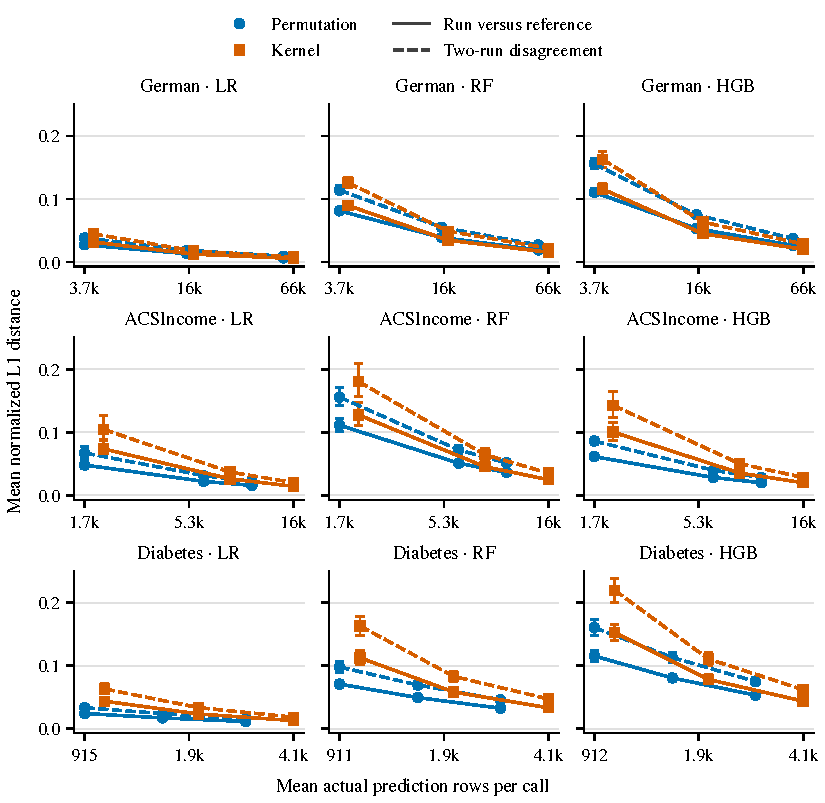
\includegraphics[width=\linewidth]{figures/error_repeatability.pdf}
\caption[Reference accuracy and repeat-run disagreement on a matched scale.]{Run-reference error and two-run disagreement use the same denominator, max(exact-reference L1,0.01 probability units). Run-reference distances average 30 runs per input; two-run distances average all distinct run pairs once per input, then equally over 60 independent inputs. Supplied pointwise 95\% instance-cluster percentile intervals are conditional on the fitted model, split and background. Two-run disagreement is not single-run accuracy; equality of the curves does not validate an explanation. Horizontal positions are mean measured prediction rows per single call. Both methods target the same empirical interventional probability game over grouped raw features with B=32.
}
\label{fig:error-repeatability}
\end{figure}
\clearpage
\begin{figure}[tb]
\centering
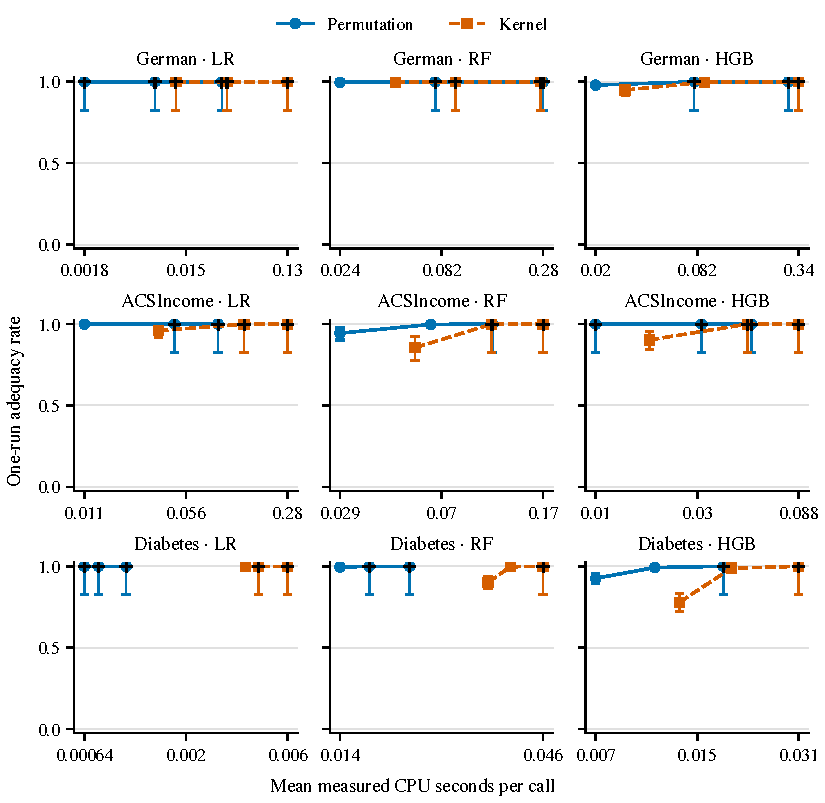
\includegraphics[width=\linewidth]{figures/budget_cpu.pdf}
\caption[Complete main-panel budget cpu.]{One-run adequacy: normalized L1 error $\leq$0.20 and signed top-3 overlap $\geq$2/3 against the exact finite-game reference. L1 normalization is max(reference L1,0.01 probability units). For each fixed fitted model, 60 held-out inputs and 30 independent runs per input, estimator and requested budget; background B=32. The target is positive-class probability for the fixed empirical interventional game over grouped raw features. Estimates average equally over inputs and runs. Bars are analysis-supplied pointwise 95\% instance-cluster percentile intervals, conditional on the fitted model, split and background. Black plus markers identify observed all-zero/all-one panels whose displayed bars instead use the supplied two-sided 95\% bounded-instance Hoeffding interval. These are observed rates and descriptive intervals, not population 95\% adequacy certification. Horizontal positions are mean measured per-call process CPU time, excluding training and reference computation. CPU is the main timing comparison because recorded wall time contains severe execution interruptions.
}
\label{fig:budget-cpu}
\end{figure}
\clearpage
\begin{figure}[tb]
\centering
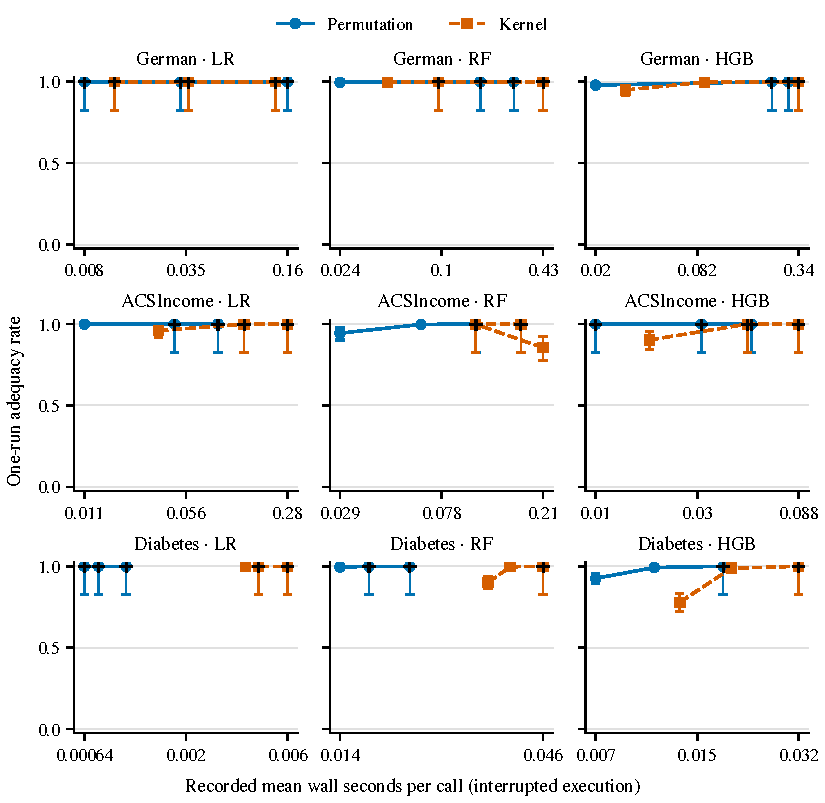
\includegraphics[width=\linewidth]{figures/budget_time.pdf}
\caption[Complete main-panel budget time.]{One-run adequacy: normalized L1 error $\leq$0.20 and signed top-3 overlap $\geq$2/3 against the exact finite-game reference. L1 normalization is max(reference L1,0.01 probability units). For each fixed fitted model, 60 held-out inputs and 30 independent runs per input, estimator and requested budget; background B=32. The target is positive-class probability for the fixed empirical interventional game over grouped raw features. Estimates average equally over inputs and runs. Bars are analysis-supplied pointwise 95\% instance-cluster percentile intervals, conditional on the fitted model, split and background. Black plus markers identify observed all-zero/all-one panels whose displayed bars instead use the supplied two-sided 95\% bounded-instance Hoeffding interval. These are observed rates and descriptive intervals, not population 95\% adequacy certification. Horizontal positions are mean measured per-call wall time, excluding training and reference computation. Severe execution interruptions and shared-host scheduling are retained. These are execution records, not deployment-latency benchmarks or latency quantiles; use CPU/actual-row curves for efficiency comparison.
}
\label{fig:budget-time}
\end{figure}
\clearpage
\begin{figure}[tb]
\centering
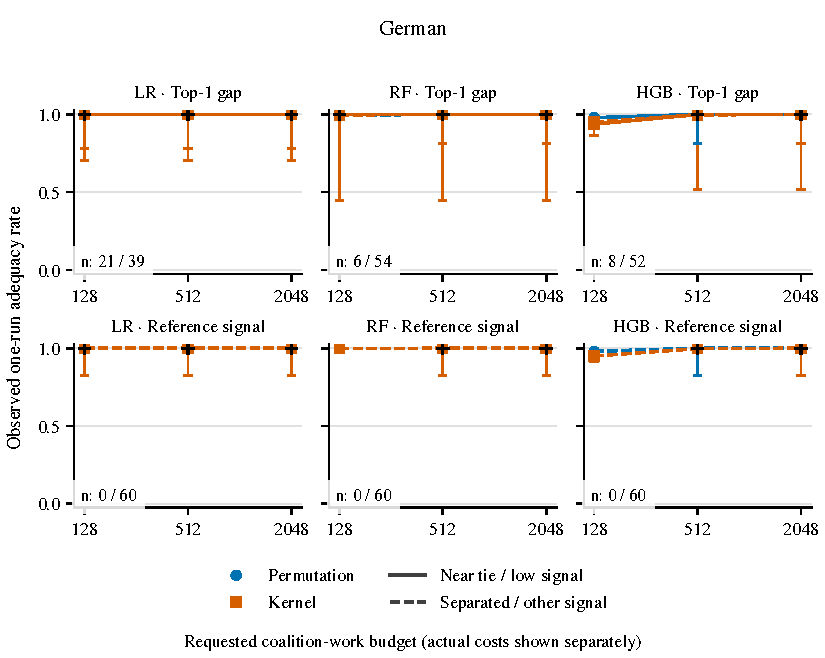
\includegraphics[width=\linewidth]{figures/conditions_german.pdf}
\caption[Complete main-panel conditions german.]{Reference-defined conditions for German. Upper row: near-top-1 tie versus separated, using (largest minus second-largest absolute reference attribution)/max(reference L1,0.01) $\leq$0.02. Lower row: low signal (reference L1 <0.01 probability units) versus other signal. Each panel labels independent-input counts in solid/dashed order; counts do not multiply across runs or budgets. Empty strata have no estimate; singleton strata show the observed estimate without an interval. Adequacy requires normalized L1 $\leq$0.20 and signed top-3 overlap $\geq$2/3. These descriptive strata are fixed by the exact reference, not selected using explanation performance. No main input has low signal, so that empty stratum is untested rather than a zero-success finding. Requested work labels do not compare equal actual work. Each input has 30 independent runs per estimator/budget; the fixed 32-row empirical interventional probability game uses grouped raw features. Bars are analysis-supplied pointwise 95\% instance-cluster percentile intervals, conditional on the fitted model, split and background. Black plus markers denote observed all-zero/all-one panels using the supplied two-sided 95\% bounded-instance Hoeffding interval instead. Interior intervals are descriptive approximations. No population $\geq$0.95 or individual-input certification follows from the plotted rates.
}
\label{fig:conditions-german}
\end{figure}
\clearpage
\begin{figure}[tb]
\centering
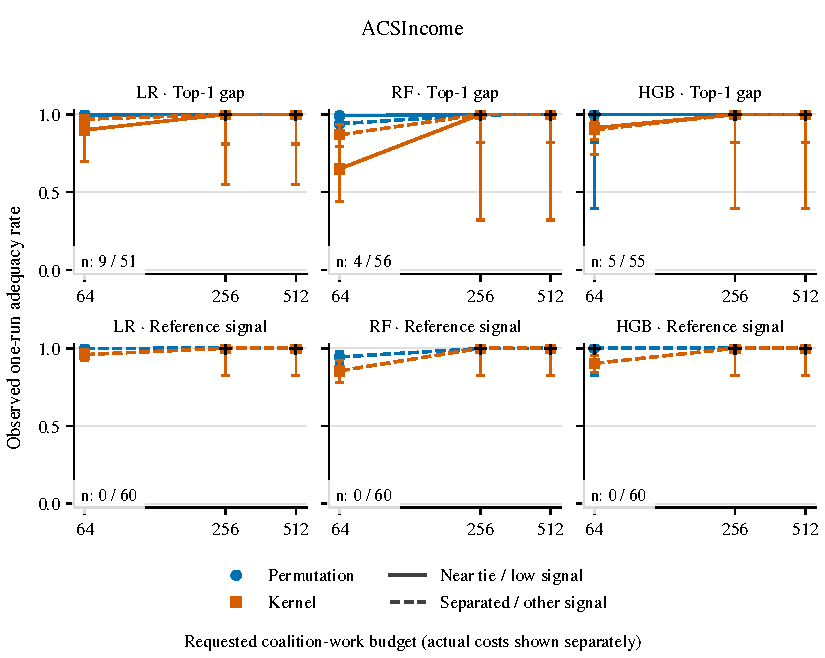
\includegraphics[width=\linewidth]{figures/conditions_acs.pdf}
\caption[Complete main-panel conditions acs.]{Reference-defined conditions for ACSIncome. Upper row: near-top-1 tie versus separated, using (largest minus second-largest absolute reference attribution)/max(reference L1,0.01) $\leq$0.02. Lower row: low signal (reference L1 <0.01 probability units) versus other signal. Each panel labels independent-input counts in solid/dashed order; counts do not multiply across runs or budgets. Empty strata have no estimate; singleton strata show the observed estimate without an interval. Adequacy requires normalized L1 $\leq$0.20 and signed top-3 overlap $\geq$2/3. These descriptive strata are fixed by the exact reference, not selected using explanation performance. No main input has low signal, so that empty stratum is untested rather than a zero-success finding. Requested work labels do not compare equal actual work. Each input has 30 independent runs per estimator/budget; the fixed 32-row empirical interventional probability game uses grouped raw features. Bars are analysis-supplied pointwise 95\% instance-cluster percentile intervals, conditional on the fitted model, split and background. Black plus markers denote observed all-zero/all-one panels using the supplied two-sided 95\% bounded-instance Hoeffding interval instead. Interior intervals are descriptive approximations. No population $\geq$0.95 or individual-input certification follows from the plotted rates.
}
\label{fig:conditions-acs}
\end{figure}
\clearpage
\begin{figure}[tb]
\centering
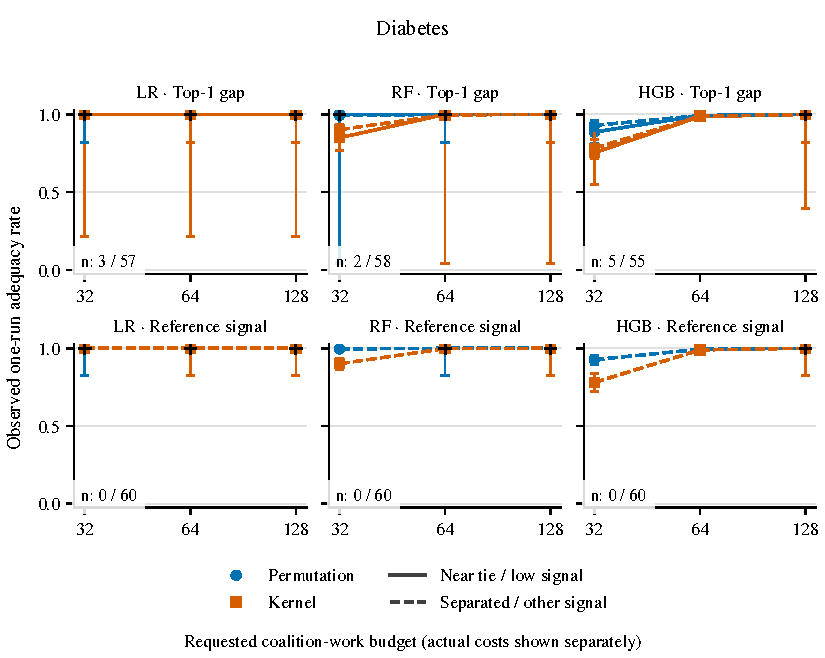
\includegraphics[width=\linewidth]{figures/conditions_diabetes.pdf}
\caption[Complete main-panel conditions diabetes.]{Reference-defined conditions for Diabetes. Upper row: near-top-1 tie versus separated, using (largest minus second-largest absolute reference attribution)/max(reference L1,0.01) $\leq$0.02. Lower row: low signal (reference L1 <0.01 probability units) versus other signal. Each panel labels independent-input counts in solid/dashed order; counts do not multiply across runs or budgets. Empty strata have no estimate; singleton strata show the observed estimate without an interval. Adequacy requires normalized L1 $\leq$0.20 and signed top-3 overlap $\geq$2/3. These descriptive strata are fixed by the exact reference, not selected using explanation performance. No main input has low signal, so that empty stratum is untested rather than a zero-success finding. Requested work labels do not compare equal actual work. Each input has 30 independent runs per estimator/budget; the fixed 32-row empirical interventional probability game uses grouped raw features. Bars are analysis-supplied pointwise 95\% instance-cluster percentile intervals, conditional on the fitted model, split and background. Black plus markers denote observed all-zero/all-one panels using the supplied two-sided 95\% bounded-instance Hoeffding interval instead. Interior intervals are descriptive approximations. No population $\geq$0.95 or individual-input certification follows from the plotted rates.
}
\label{fig:conditions-diabetes}
\end{figure}
\clearpage
\begin{figure}[tb]
\centering
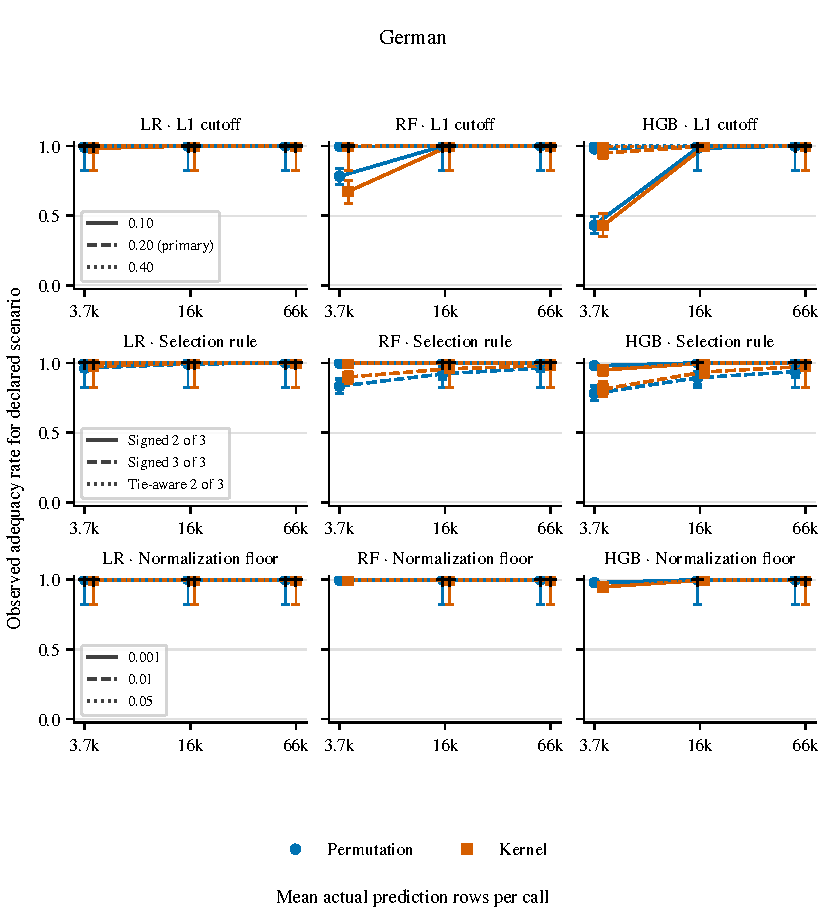
\includegraphics[width=\linewidth]{figures/metric_sensitivity_german.pdf}
\caption[Complete main-panel metric sensitivity german.]{Predeclared adequacy scenarios for German; no scenario is selected after seeing the rates. Top row varies the normalized L1 cutoff (0.10/0.20/0.40), retaining signed top-3 overlap $\geq$2/3 and floor 0.01. Middle row fixes cutoff 0.20/floor 0.01 and compares signed overlap $\geq$2/3 (primary), all three matching signed features, and the analysis-defined 1e-6 probability-unit tie-aware selection rule. Bottom row varies normalization floor (0.001/0.01/0.05 probability units) in max(reference L1,floor), retaining cutoff 0.20 and the same primary signed-top-3 event. These floors change the metric, not the target or explanation calls. All main reference norms exceed 0.05, so these floor curves coincide; weak-signal behavior is untested. Curves use the same runs and are correlated. Each input has 30 independent runs per estimator/budget; the fixed 32-row empirical interventional probability game uses grouped raw features. Bars are analysis-supplied pointwise 95\% instance-cluster percentile intervals, conditional on the fitted model, split and background. Black plus markers denote observed all-zero/all-one panels using the supplied two-sided 95\% bounded-instance Hoeffding interval instead. Interior intervals are descriptive approximations. No population $\geq$0.95 or individual-input certification follows from the plotted rates.
}
\label{fig:metric-sensitivity-german}
\end{figure}
\clearpage
\begin{figure}[tb]
\centering
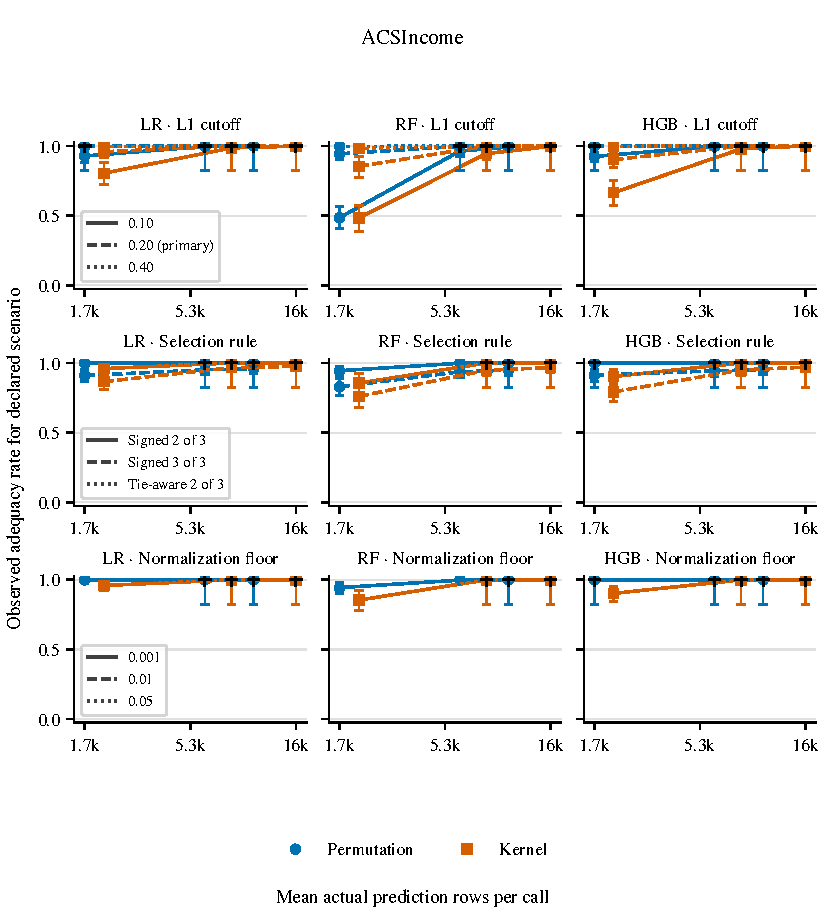
\includegraphics[width=\linewidth]{figures/metric_sensitivity_acs.pdf}
\caption[Complete main-panel metric sensitivity acs.]{Predeclared adequacy scenarios for ACSIncome; no scenario is selected after seeing the rates. Top row varies the normalized L1 cutoff (0.10/0.20/0.40), retaining signed top-3 overlap $\geq$2/3 and floor 0.01. Middle row fixes cutoff 0.20/floor 0.01 and compares signed overlap $\geq$2/3 (primary), all three matching signed features, and the analysis-defined 1e-6 probability-unit tie-aware selection rule. Bottom row varies normalization floor (0.001/0.01/0.05 probability units) in max(reference L1,floor), retaining cutoff 0.20 and the same primary signed-top-3 event. These floors change the metric, not the target or explanation calls. All main reference norms exceed 0.05, so these floor curves coincide; weak-signal behavior is untested. Curves use the same runs and are correlated. Each input has 30 independent runs per estimator/budget; the fixed 32-row empirical interventional probability game uses grouped raw features. Bars are analysis-supplied pointwise 95\% instance-cluster percentile intervals, conditional on the fitted model, split and background. Black plus markers denote observed all-zero/all-one panels using the supplied two-sided 95\% bounded-instance Hoeffding interval instead. Interior intervals are descriptive approximations. No population $\geq$0.95 or individual-input certification follows from the plotted rates.
}
\label{fig:metric-sensitivity-acs}
\end{figure}
\clearpage
\begin{figure}[tb]
\centering
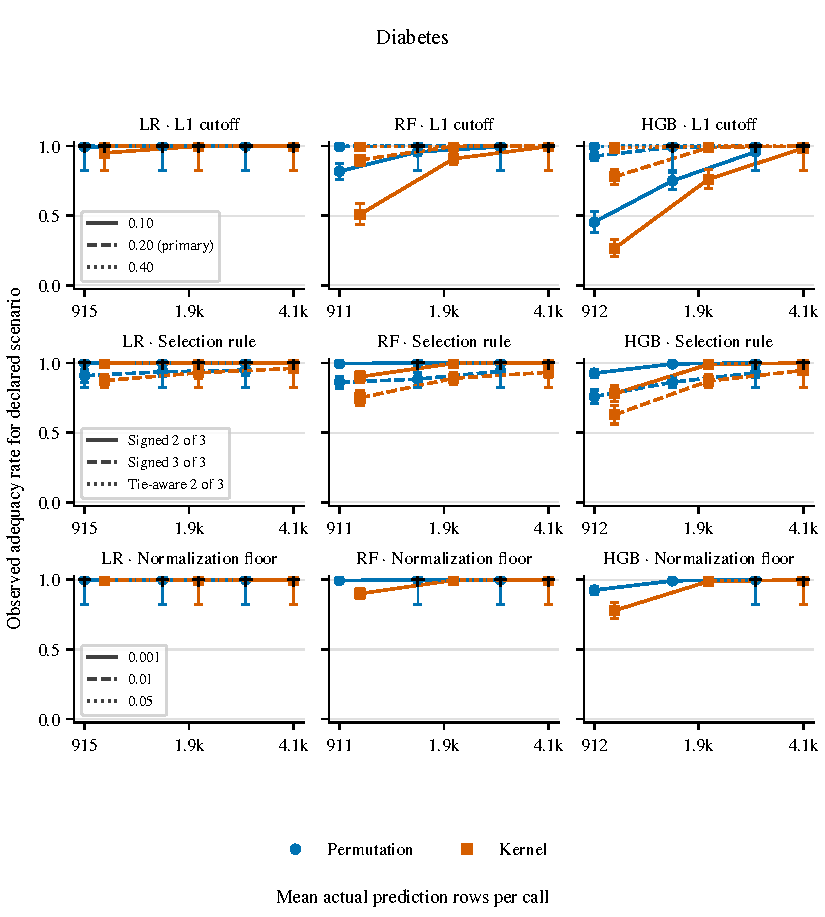
\includegraphics[width=\linewidth]{figures/metric_sensitivity_diabetes.pdf}
\caption[Complete main-panel metric sensitivity diabetes.]{Predeclared adequacy scenarios for Diabetes; no scenario is selected after seeing the rates. Top row varies the normalized L1 cutoff (0.10/0.20/0.40), retaining signed top-3 overlap $\geq$2/3 and floor 0.01. Middle row fixes cutoff 0.20/floor 0.01 and compares signed overlap $\geq$2/3 (primary), all three matching signed features, and the analysis-defined 1e-6 probability-unit tie-aware selection rule. Bottom row varies normalization floor (0.001/0.01/0.05 probability units) in max(reference L1,floor), retaining cutoff 0.20 and the same primary signed-top-3 event. These floors change the metric, not the target or explanation calls. All main reference norms exceed 0.05, so these floor curves coincide; weak-signal behavior is untested. Curves use the same runs and are correlated. Each input has 30 independent runs per estimator/budget; the fixed 32-row empirical interventional probability game uses grouped raw features. Bars are analysis-supplied pointwise 95\% instance-cluster percentile intervals, conditional on the fitted model, split and background. Black plus markers denote observed all-zero/all-one panels using the supplied two-sided 95\% bounded-instance Hoeffding interval instead. Interior intervals are descriptive approximations. No population $\geq$0.95 or individual-input certification follows from the plotted rates.
}
\label{fig:metric-sensitivity-diabetes}
\end{figure}
\clearpage
\begin{figure}[tb]
\centering
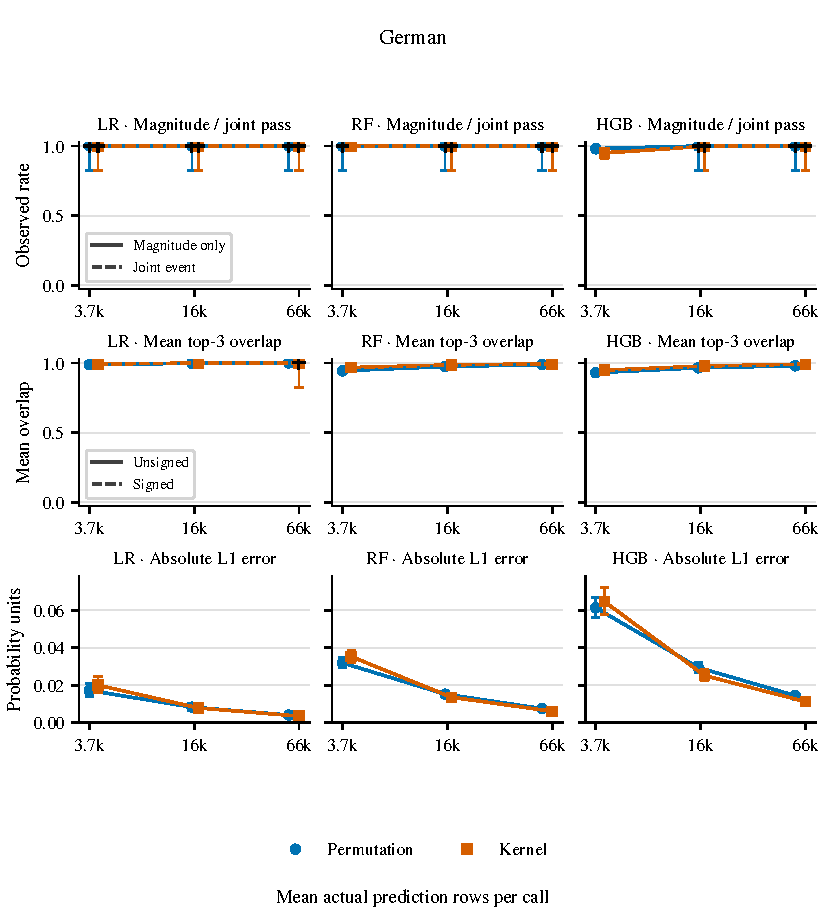
\includegraphics[width=\linewidth]{figures/accuracy_components_german.pdf}
\caption[Complete main-panel accuracy components german.]{Accuracy components for German. Upper row compares the normalized-magnitude pass probability (L1/max(reference L1,0.01) $\leq$0.20) with the primary joint event, which additionally requires signed top-3 overlap $\geq$2/3. Middle row gives mean unsigned and signed top-3 overlap (matching features or feature-sign tokens, divided by three); these are average overlaps, not pass probabilities. Lower row shows mean absolute L1 error against the exact reference in probability units, without division by the attribution norm. Each input has 30 independent runs per estimator/budget; the fixed 32-row empirical interventional probability game uses grouped raw features. Bars are analysis-supplied pointwise 95\% instance-cluster percentile intervals, conditional on the fitted model, split and background. Black plus markers denote observed all-zero/all-one panels using the supplied two-sided 95\% bounded-instance Hoeffding interval instead. Interior intervals are descriptive approximations. No population $\geq$0.95 or individual-input certification follows from the plotted rates.
}
\label{fig:accuracy-components-german}
\end{figure}
\clearpage
\begin{figure}[tb]
\centering
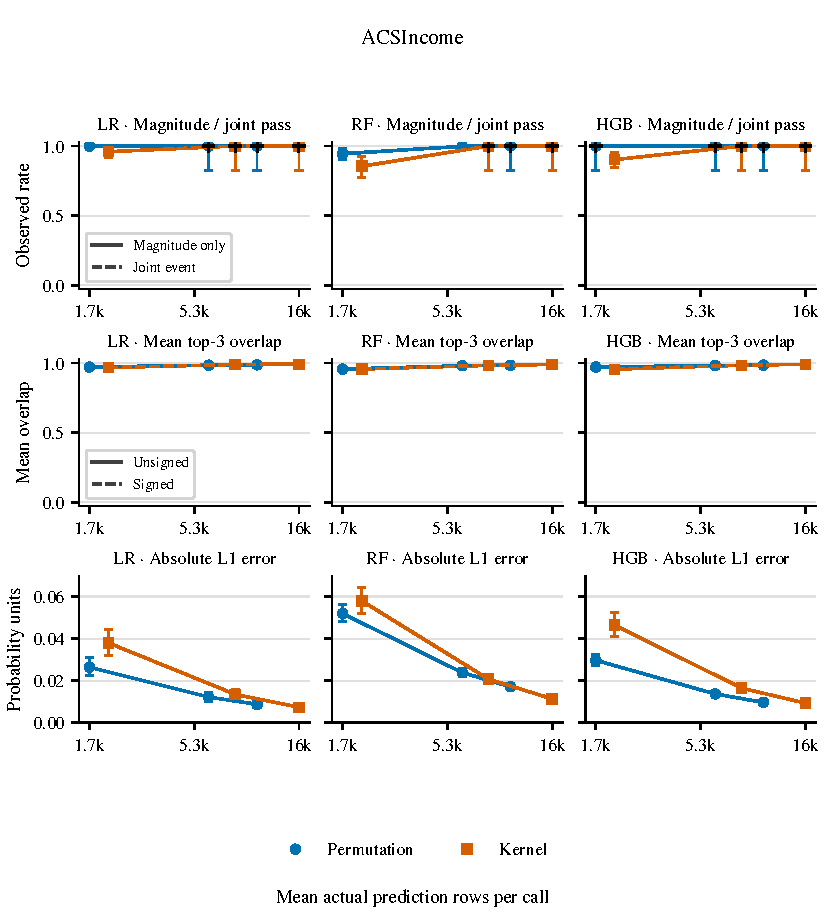
\includegraphics[width=\linewidth]{figures/accuracy_components_acs.pdf}
\caption[Complete main-panel accuracy components acs.]{Accuracy components for ACSIncome. Upper row compares the normalized-magnitude pass probability (L1/max(reference L1,0.01) $\leq$0.20) with the primary joint event, which additionally requires signed top-3 overlap $\geq$2/3. Middle row gives mean unsigned and signed top-3 overlap (matching features or feature-sign tokens, divided by three); these are average overlaps, not pass probabilities. Lower row shows mean absolute L1 error against the exact reference in probability units, without division by the attribution norm. Each input has 30 independent runs per estimator/budget; the fixed 32-row empirical interventional probability game uses grouped raw features. Bars are analysis-supplied pointwise 95\% instance-cluster percentile intervals, conditional on the fitted model, split and background. Black plus markers denote observed all-zero/all-one panels using the supplied two-sided 95\% bounded-instance Hoeffding interval instead. Interior intervals are descriptive approximations. No population $\geq$0.95 or individual-input certification follows from the plotted rates.
}
\label{fig:accuracy-components-acs}
\end{figure}
\clearpage
\begin{figure}[tb]
\centering
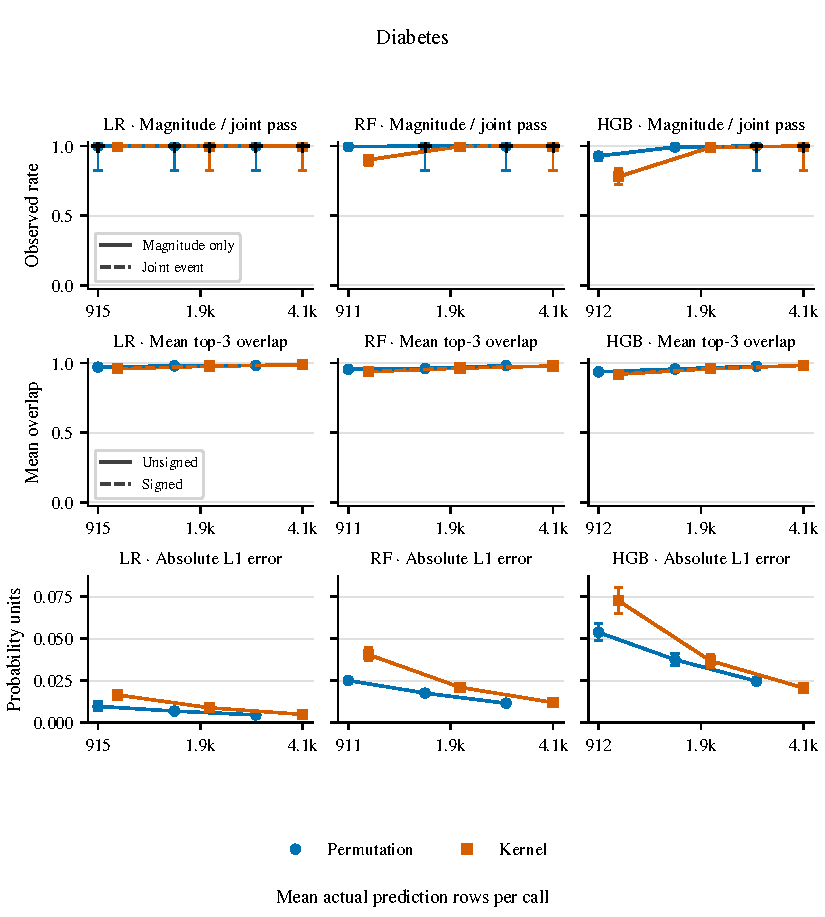
\includegraphics[width=\linewidth]{figures/accuracy_components_diabetes.pdf}
\caption[Complete main-panel accuracy components diabetes.]{Accuracy components for Diabetes. Upper row compares the normalized-magnitude pass probability (L1/max(reference L1,0.01) $\leq$0.20) with the primary joint event, which additionally requires signed top-3 overlap $\geq$2/3. Middle row gives mean unsigned and signed top-3 overlap (matching features or feature-sign tokens, divided by three); these are average overlaps, not pass probabilities. Lower row shows mean absolute L1 error against the exact reference in probability units, without division by the attribution norm. Each input has 30 independent runs per estimator/budget; the fixed 32-row empirical interventional probability game uses grouped raw features. Bars are analysis-supplied pointwise 95\% instance-cluster percentile intervals, conditional on the fitted model, split and background. Black plus markers denote observed all-zero/all-one panels using the supplied two-sided 95\% bounded-instance Hoeffding interval instead. Interior intervals are descriptive approximations. No population $\geq$0.95 or individual-input certification follows from the plotted rates.
}
\label{fig:accuracy-components-diabetes}
\end{figure}
\clearpage
\begin{figure}[tb]
\centering
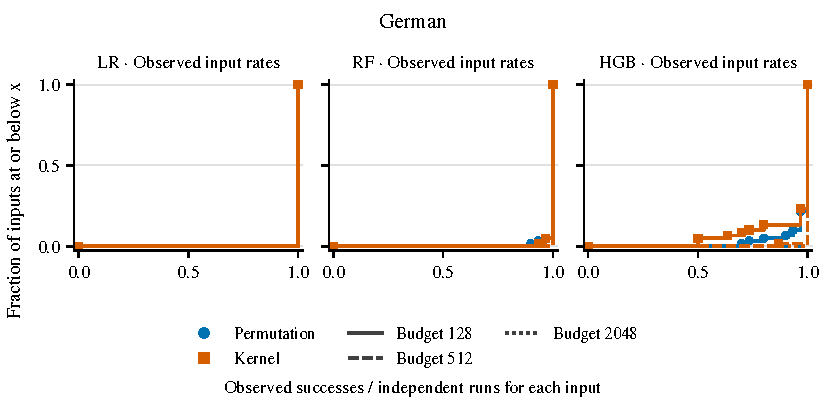
\includegraphics[width=\linewidth]{figures/instance_distribution_german.pdf}
\caption[Complete main-panel instance distribution german.]{Per-input heterogeneity for German: empirical cumulative distribution of the observed primary-event success fractions among 60 inputs per fitted model, each measured with 30 independent runs per estimator/budget. The event requires L1/max(exact-reference L1,0.01) $\leq$0.20 and signed top-3 overlap $\geq$2/3. Each input contributes once to each curve; vertical masses at zero/one are retained. Curves describe observed finite-run fractions, not the distribution of known true per-input success probabilities. There are no confidence bands or individual-input certifications: even no observed failures in these runs does not establish a 0.95 success probability. Budget labels are requested work, with actual-work/time comparisons supplied separately. The fixed B=32 empirical interventional probability game uses grouped raw features; split/model/background remain fixed.
}
\label{fig:instance-distribution-german}
\end{figure}
\clearpage
\begin{figure}[tb]
\centering
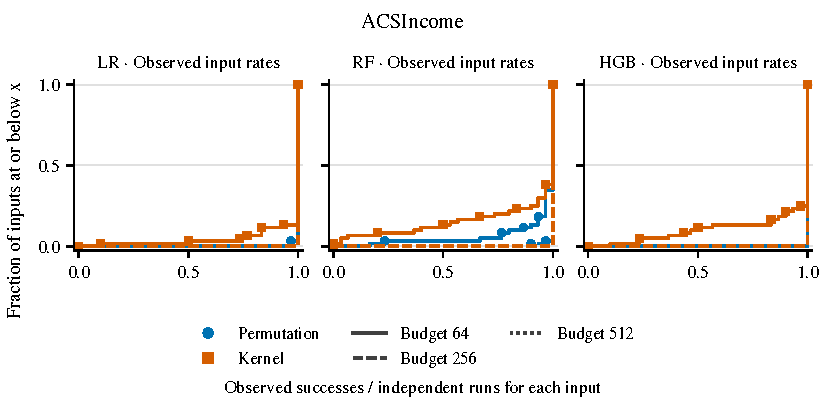
\includegraphics[width=\linewidth]{figures/instance_distribution_acs.pdf}
\caption[Complete main-panel instance distribution acs.]{Per-input heterogeneity for ACSIncome: empirical cumulative distribution of the observed primary-event success fractions among 60 inputs per fitted model, each measured with 30 independent runs per estimator/budget. The event requires L1/max(exact-reference L1,0.01) $\leq$0.20 and signed top-3 overlap $\geq$2/3. Each input contributes once to each curve; vertical masses at zero/one are retained. Curves describe observed finite-run fractions, not the distribution of known true per-input success probabilities. There are no confidence bands or individual-input certifications: even no observed failures in these runs does not establish a 0.95 success probability. Budget labels are requested work, with actual-work/time comparisons supplied separately. The fixed B=32 empirical interventional probability game uses grouped raw features; split/model/background remain fixed.
}
\label{fig:instance-distribution-acs}
\end{figure}
\clearpage
\begin{figure}[tb]
\centering
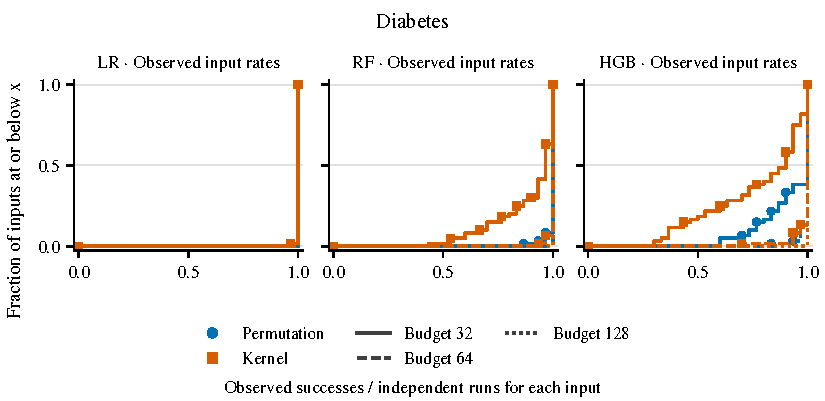
\includegraphics[width=\linewidth]{figures/instance_distribution_diabetes.pdf}
\caption[Complete main-panel instance distribution diabetes.]{Per-input heterogeneity for Diabetes: empirical cumulative distribution of the observed primary-event success fractions among 60 inputs per fitted model, each measured with 30 independent runs per estimator/budget. The event requires L1/max(exact-reference L1,0.01) $\leq$0.20 and signed top-3 overlap $\geq$2/3. Each input contributes once to each curve; vertical masses at zero/one are retained. Curves describe observed finite-run fractions, not the distribution of known true per-input success probabilities. There are no confidence bands or individual-input certifications: even no observed failures in these runs does not establish a 0.95 success probability. Budget labels are requested work, with actual-work/time comparisons supplied separately. The fixed B=32 empirical interventional probability game uses grouped raw features; split/model/background remain fixed.
}
\label{fig:instance-distribution-diabetes}
\end{figure}
\clearpage
